% vim: tw=80

\chapter{Theoretical Foundations}
\label{sec:theoretical_foundations}

A deeper understanding of physical principles always results from the interplay
of experimental measurements and the corresponding theoretical predictions.
Theoretical models attempt to describe nature's behavior and must be excluded or
tentatively confirmed in precise experiments. In the second half of the 20th
century, theoretical and experimental physicists have made great progress in
describing the fundamental particles and their interactions in a self-consistent
model which is today established as the Standard Model of particle physics (SM).

This chapter shortly summarizes the Standard Model while concentrating on
quantum chromodynamics (QCD) and those properties, which are the theoretical
foundations of this thesis. More extensive and profound discussions can be found
in~\cite{Peskin:1995ev,Agashe:2014kda,Ellis:1991qj,Buckley:2011ms}.

Throughout this thesis, the common unit convention in particle physics is used.
It is based on SI units, but is supplemented with the units electron volt
(\si{\electronvolt}) for energy and barn (\si{\barn}) for the interaction cross
section. Furthermore, the speed of light $c$ and the reduced Planck constant
$\hbar$ are set to unity,
%
\begin{equation*}
    c = \hbar = 1.
\end{equation*}

\section{Standard Model of Particle Physics}

The Standard Model of particle physics is a comprehensive theory  which
describes the fundamental particles and their interactions from first
principles. The SM is founded on the concept of quantum field theories, in which
the elementary particles and the interactions between them are described by
quantized gauge fields. There are four fundamental forces of which three are
considered in the SM. While the predictions of the SM have been demonstrated to
be extremely robust in a huge variety of experiments, it falls short of being a
complete theory of everything, as it does not include a description of the
gravitational force and can describe neither dark matter nor non-zero neutrino
masses resulting from neutrino oscillations.

Each of the fundamental spin-\sfrac{1}{2} particles, also known as fermions, has
a corresponding antiparticle with the same properties but opposite-sign quantum
numbers. They are classified into three families and carry quantum numbers of
electric charge $Q$, weak isospin $T$ and color. The weak hypercharge $Y_W$ is
related to the weak isospin and the electric charge by $Y_W = 2(Q-T_3)$.

The electromagnetic and weak forces are described by a U(1)$\times$SU(2)
symmetry which is spontaneously broken by the coupling to the scalar Higgs
field. The gauge bosons of the unified electroweak theory are a mixture of the
gauge bosons of the unbroken symmetry resulting in the massive $W^\pm$ and $Z^0$
bosons and the massless photon. The eigenstates of the weak interaction differ
from the mass eigenstates and can be calculated by rotating the mass eigenstates
using the CKM matrix~\cite{Cabibbo:1963yz,Kobayashi:1973fv}. The same effect is
observed in the lepton sector in which the mass eigenstates of the neutrinos do
not match the interaction eigenstates leading to oscillations between neutrino
flavors.  The analogous matrix is called PMNS
matrix~\cite{Maki:1962mu,Pontecorvo:1957qd}.

The strong force is described by the unbroken $\mathrm{SU}(3)$ color gauge
theory~\cite{Zweig:1981pd,Fritzsch:1973pi}, called quantum chromodynamics. The
eight gauge bosons of the theory, called gluons, carry color charge. 

The Higgs boson, the field quantum of the Higgs field responsible for
electroweak symmetry breaking, had long been postulated by theoretical models
until its recent discovery at the LHC~\cite{Chatrchyan:2012xdj,Aad:2012tfa}.

\section{Quantum Chromodynamics}

Quantum chromodynamics is the gauge field theory that describes the
strong interaction of quarks and gluons. The gauge group of the theory is the
special unitary group SU(3). The QCD Lagrangian is given by

\begin{equation*}
   \mathcal{L} = \sum_q \bar \psi_{q,a} \left( i \gamma^\mu \partial_\mu
   \delta_{ab} - g_s \gamma^\mu t_{ab}^C \mathcal{A}_{\mu}^C - m_q \delta_{ab}
   \right) \psi_{q,b} - \frac{1}{4} F_{\mu\nu}^{A} F^{A \mu\nu},
\end{equation*}
%
where $\gamma_\mu$ are the Dirac $\gamma$-matrices and $\psi_{q,a}$ are quark-field
spinors for a quark with flavor $q$, mass $m_q$ and a color of index $a$
which runs from $1$ to $N_C=3$. The $t_{ab}^C$ correspond to the eight
$3\times3$ matrices and are the generators of the $\mathrm{SU}(3)$
group.$\mathcal{A}_\mu^C$ denotes the gluon fields and $C$ runs from 1 to
$N_C-1$, resulting in eight different gluons. The QCD coupling strength is defined
by $g_s$. The field tensor $F_{\mu\nu}^A$ is given by

\begin{equation*}
    F_{\mu\nu}^A = \partial_\mu \mathcal{A}_\nu^A - \partial_{\nu}
    \mathcal{A}_{\mu}^A - g_s f_{ABC} \mathcal{A}_{\mu}^B
    \mathcal{A}_{\nu}^C
\end{equation*}
%
where $f_{ABC}$ are the structure constants of the SU(3) group. The last term of
the field tensor originates from the non-abelian structure, where the generators
do not commute, but obey the relation

\begin{equation*}
    \left[t^A, t^B \right] = if_{ABC} t^{C}.
\end{equation*}
%
This leads to the self-coupling of gluons, one of the prominent features of QCD,
resulting in three and four gluon vertex interactions. The fundamental
interaction vertices of QCD can be illustrated by the Feynman diagrams in
Fig.~\ref{fig:fundamental_couplings}. The complete QCD Lagrangian also includes
a gauge-fixing term and the Faddeev-Popov ghost fields~\cite{Faddeev:1967fc},
which are not further discussed in this thesis.

\begin{figure}[htb] 
    \centering
    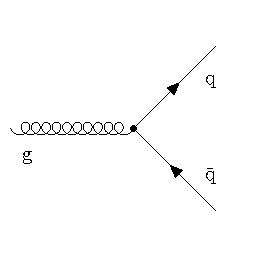
\includegraphics[width=0.33\textwidth]{figures/drawings/feynman/gqq.pdf}\hfill
    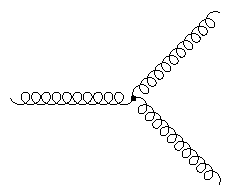
\includegraphics[width=0.33\textwidth]{figures/drawings/feynman/ggg.pdf}\hfill
    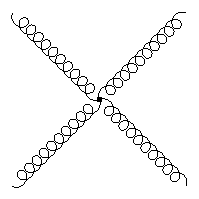
\includegraphics[width=0.33\textwidth]{figures/drawings/feynman/gggg.pdf}\hfill
    \caption[Fundamental vertices of QCD]{The fundamental Feynman rules of QCD
    comprise a quark-antiquark-gluon vertex, a three-gluon vertex and a four-gluon
    vertex. The first two are proportional to $g_{s}$, the last one is
    proportional to $g_{s}^2$.} 
    \label{fig:fundamental_couplings} 
\end{figure}

Unlike the other fundamental forces, the strong force exhibits two unique and
opposing features. Experiments show that quarks and gluons behave like free
particles at high energies or small distances. This is called \emph{asymptotic
freedom} and is described in QCD by the decreasing of the strong coupling at
high energies. At low energies however, quarks and gluons cannot be observed as
free particles at larger distances. The strong coupling increases with distance
and the creation of new quark-antiquark pairs from the vacuum is energetically
favored at some point. This phenomenon, called \emph{confinement}, implies that
the strong coupling increases at low energies and is divergent. Consequently,
perturbative QCD is not applicable in this energy regime.

\subsection{Perturbative QCD}

All observables $X$ in perturbative QCD (pQCD) are developed as a
perturbative series in powers of the strong coupling \as:

\begin{equation*}
    X = \sum_{n=0}^N \as^n c_i = c_0 + \as^1 c_1 + \as^2 c_2 + \ldots, 
\end{equation*}
%
where $c_i$ are the perturbative coefficients. The expansion already yields
sufficiently accurate results after the first orders of the perturbative series
if $\as \ll 1$ so that the series converges quickly. However, several features
complicate perturbative calculations. Ultraviolet (UV) divergences enter the
calculations beyond leading order due to loop corrections. The divergences can
be removed by a procedure called renormalization which is described in
Sec.~\ref{sec:renormalization}. Soft and collinear divergences also need to be
handled in perturbative calculations. They arise from singularities at
phase-space boundaries and neglected quark masses. Observables need to be
defined to be infrared safe and short-distance effects need to be separated from
the divergent long-range part, which can be absorbed into the PDFs in a
procedure called \emph{collinear factorization}, detailed in
Sec.~\ref{sec:factorization}.

\subsection{Renormalization and Running of the Strong Coupling}
\label{sec:renormalization}

Beyond leading order, the calculations include loop corrections which result in
UV divergences when calculating the momenta integrals of the loops. To make the
result finite, a renormalization procedure is applied. It introduces the
renormalization scale \mur. There are different renormalization schemes, of
which the $\overline{\mathrm{MS}}$ scheme~\cite{Weinberg:1951ss,tHooft:1973mm}
is the most popular. Consequently, the observable $X$ and the strong coupling
become functions of \mur. 

Nonetheless, the observable $X$ may not depend on the arbitrarily chosen \mur.
The renormalization group equation (RGE) states that the dependence of $X$ on
\mur must cancel. This can be mathematically expressed by

\begin{equation} 
    \mur^2 \frac{d}{d \mur^2} X \left(\frac{Q^2}{\mur^2},\as(\mur^2)\right) = \left(
    \mur^2 \frac{\partial X}{\partial \mur^2} + \mur^2 \frac{\partial
    \as(\mu^2)}{\partial \mur^2} \frac{\partial X}{\partial \as(\mu^2)} \right) \stackrel{!}{=} 0 
\end{equation}
%
and states that any dependence of $X$ on \mur must be canceled by the
\mur-depedence of \as. Thus, the strong coupling has to fulfill the
equation

\begin{equation}
    \mur^2 \frac{d \as}{d \mur^2} = \beta(\as) = - \left( \beta_0 \as^2 + \beta_1 \as^3
    + \beta_2 \as^4 + \ldots \right)
    \label{eq:as_rge}
\end{equation}
%
where $\beta_0$, $\beta_1$ and $\beta 2$ are the 1-loop, 2-loop and 3-loop 
$\beta$-function coefficients, which encode the the dependence of the coupling
on the energy scale. They are given for the coupling of an effective
theory, in which the $n_f$ quark flavors are light ($m_q \ll \mur$). Here, they
are given in the $\overline{\mathrm{MS}}$ scheme:

\begin{equation} 
    \beta_0 = \frac{33 - 2 n_f}{12\pi},
\end{equation}

\begin{equation} 
    \beta_1 = \frac{153 - 19 n_f}{24\pi^2},
\end{equation}

\begin{equation} 
   \beta_2 = \frac{2857 -\left(\sfrac{5033}{9}\right)n_f + \left(\sfrac{335}{27}
   \right)n_f^2}{128 \pi^3}.
\end{equation}
%
By integrating Eq.~\ref{eq:as_rge}, the energy dependence of \as is yielded.
Working in an energy range of constant number of flavors \ie if no quark mass
thresholds are passed, an analytic solution exists in 1-loop approximation. 

\begin{equation*}
   \as(\mur^2) = \frac{1}{\beta_0 \ln \left( \sfrac{\mur^2}{\Lambda^2} \right)}
\end{equation*}

$\Lambda$ is the constant of integration and corresponds to the scale at which
the perturbative coupling would become large and the perturbative series
diverge. It is very often convenient to give the strong coupling at a specific
scale, from which the coupling at any scale is calculated. It is common practice
to report \asmz, the strong coupling at the scale of the Z boson mass. Thus, the
1-loop analytical function can be expressed as

\begin{equation*}
   \as\left(\mur, \as(\mz)\right) = \frac{\as(\mz)}{1 + \as(\mz)\beta_0 \ln
       \left( \sfrac{\mur^2}{\mz^2} \right)}.
\end{equation*}

\begin{figure}[htbp] 
    \centering
    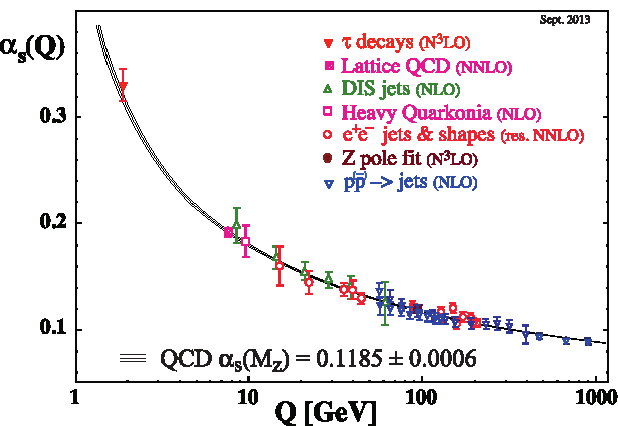
\includegraphics[width=0.95\textwidth]{figures/theoretical_foundations/as_running.pdf}\hfill
    \caption[Running of the strong coupling]{Running of the strong coupling
        constant as predicted by QCD. Determinations of the strong coupling from
        several experiments are shown at the scale of the measurement and
        confirm the running up to \SI{1}{\TeV}. Recent measurements from
        CMS~\cite{Khachatryan:2014waa,CMS:2014mna} probe the running at even
        higher scales. Figure taken from~\cite{Agashe:2014kda}.} 
    \label{fig:as_running} 
\end{figure}


As the parameter \as is a free parameter of the theory, it is deduced from
experimental measurements and evolved to the scale of the $Z$-boson. The current
world average value of the strong coupling according to the
PDG~\cite{Agashe:2014kda} reads as
%
\begin{equation*}
    \asmz = 0.1185 \pm 0.0006
\end{equation*}
%
and is determined from hadronic $\tau$ lepton decays, lattice QCD calculations,
deep inelastic scattering data, electron-positron annihilation processes and
electroweak precision fits. Fig.~\ref{fig:as_running} shows various
determinations of the strong coupling from measurements at scales $Q$,
which describe the running of the strong coupling up to the \SI{1}{\TeV} scale.

\subsection{Factorization and Parton Density Functions}
\label{sec:factorization}

The \emph{collinear factorization} factorization allows to separate the
calculation of an obserable into a short-distance part, calculable in QCD, and
an approximately but universal long-distance part, which is described by parton
distribution functions. The factorization analogously to the renormalization
involves an arbitrary choice of a factorization scale \muf. Particle emissions
with transverse momenta above \muf are included in the hard scattering
perturbative coefficients while emissions softer than \muf are accounted for
within the PDFs.

\paragraph{Parton Distribution Functions}

The structure of the proton is described by parton distribution functions (PDFs)
in which the partons represent the constituents of the proton. The PDFs give
the probability density\footnote{More specifically a number density, as the PDFs are
normalized to the number of partons.} to find a parton carrying a momentum
fraction $x$ of the proton momentum at an squared energy scale $Q^2$. As only
the $Q$-dependence is predicted by QCD, the $x$-dependence needs to be
parameterized and determined in fits to experimental data.

Several groups obtain the proton PDFs in global fits to a large variety of
measurements from different experiments. Instead of determining all (13 quark,
antiquark and gluon) PDFs independently, the number can be reduced by choosing a
sufficiently low starting scale $Q_0$ below the threshold of the charm quark
mass and calculating the heavy flavor PDFs in a heavy flavor
scheme~\cite{Thorne:2006qt}. Furthermore, the PDFs of the top and anti-top quark
are often neglected due to their large rest mass. In a fit, each parton is
parameterized with a sufficiently flexible function to describe the
$x$-dependence at the starting scale $Q_0$. The PDFs are then evolved to the 
scales of each measurement and the PDF parameters are adapted in an iterative
least-squares fit.

Global PDFs are determined by the CTEQ~\cite{Dulat:2015mca},
MMHT~\cite{Harland-Lang:2014zoa}, NNPDF~\cite{Ball:2014uwa} and the
ABM~\cite{Alekhin:2013nda} groups at LO, NLO and NNLO. While the range of
measurements which are put into the fit are often similar, there are differences
in the applied minimization method, the phenomenological approaches and the
estimation of the uncertainties. More details are given in
Sec.~\ref{sec:pdf_uncertainties}, in which the uncertainty of the PDFs on the
cross section measurement is discussed.

\begin{figure}[htbp] 
    \centering
    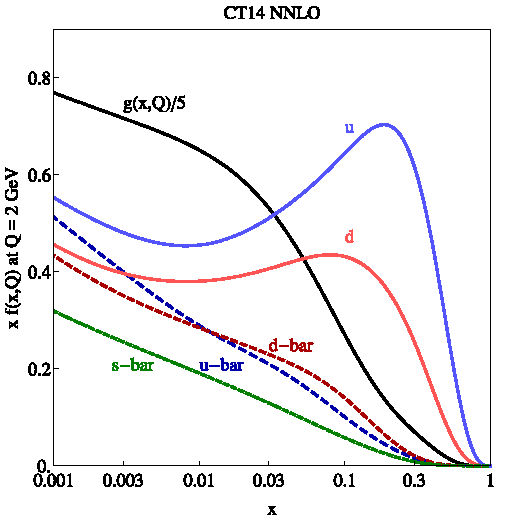
\includegraphics[width=0.49\textwidth]{figures/theoretical_foundations/ct14_2.pdf}\hfill
    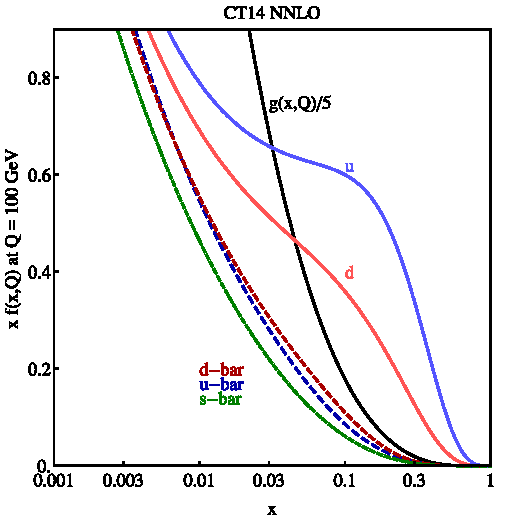
\includegraphics[width=0.49\textwidth]{figures/theoretical_foundations/ct14_100.pdf}
    \caption[CT14 NNLO PDF sets]{The CT14 NNLO PDF set with the gluon and quark
        PDFs at the scale $Q=\SI{2}{\GeV}$ (left) and evolved to $Q=\SI{100}{\GeV}$
    (right) using the DGLAP evolution equations. Figure taken
    from~\cite{Dulat:2015mca}.}
    \label{fig:ct14_parton_distributions} 
\end{figure}

The HERAPDF group~\cite{Abramowicz:2015mha} uses a slightly different approach
by using a less flexible parameterization but restricting the data to
measurements from the HERA experiments, which provide a very precise and
compatible data set. Furthermore, the HERAPDF group made their fitting framework
XFitter~\cite{Alekhin:2014irh} freely available as open-source software.
HERAFitter is employed in Sec.~\ref{sec:pdf_constraints} of this thesis to study
the constraints on the PDFs provided by the triple differential dijet
measurement.

\paragraph{DGLAP Evolution Equations}

Because of the factorization, the PDFs depend on the scale \muf. This evolution
from a scale $Q_0$ to a different scale $Q$ can be calculated using the
Dokshitzer-Gribov-Lipatov-Altarelli-Parisi
(DGLAP)~\cite{Gribov:1972ri,Altarelli:1977zs,Dokshitzer:1977sg} equations, which
have a different structure for the gluon and quark PDFs. Using the shorthand notation
%
\begin{equation*}
    \left[f \otimes P \right] = \left[ P \otimes f \right] = \int_x^1 \frac{d
    \xi}{\xi} f\left(\xi, \muf\right) P\left( \frac{x}{\xi} \right)
\end{equation*}
%
they can be expressed at leading order for the quark PDFs $q_i(x, \muf)$ as:
\begin{equation*}
    \muf \frac{\partial q_i (x, \muf)}{\partial \muf} = \left[ q_i \otimes P_{qq}
    \right] + \left[ g \otimes P_{qg} \right],
\end{equation*}
%
and for the gluon PDF $g(x, \muf)$ as
%
\begin{equation*}
    \muf \frac{\partial g (x, \muf)}{\partial \muf} = \left[\sum_i  q_i \otimes P_{gq}
    \right] + \left[g \otimes P_{gg}\right].
\end{equation*}
%
where the sum runs over all quark and antiquark flavors. $P_{ab}$ are the
so-called Altarelli-Parisi kernels, also known as splitting functions. These
give the probability to emit a parton $a$ with momentum fraction $x$ from a
parton $b$ with momentum fraction $\xi$.


\begin{figure}[htb] 
    \centering
    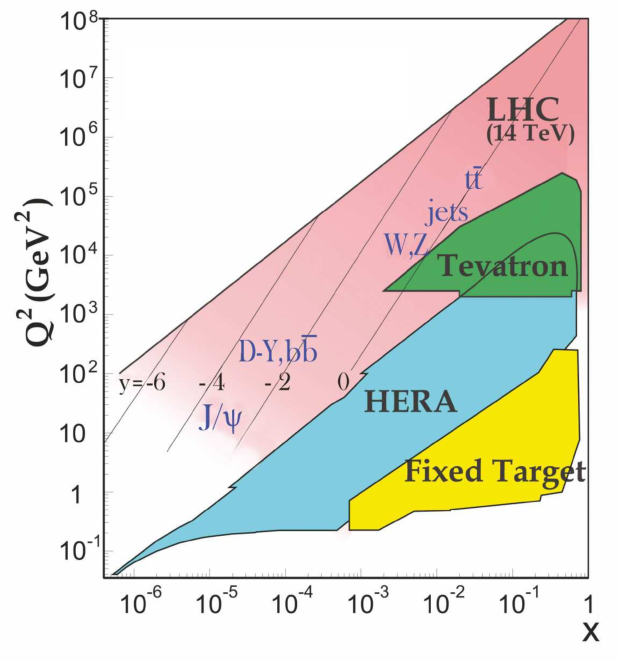
\includegraphics[width=0.8\textwidth]{figures/theoretical_foundations/phasespace.pdf}\hfill
    \caption[Kinematic phase space region of the experiments]{The phase space
        in $x$ and $Q^2$ which is accessible in current experiments.  The most
        important input for the PDFs continues to be provided by DIS
        data measured at the HERA collider. Further important constraints at
        high $x$ and low scales are provided by fixed-target experiments. The
        latest PDF sets also include LHC measurements which provide constraints
        at high energy scales $Q^2$ and high $x$ (jets, $t\bar t$) and at medium $x$
        ($W$,$Z$,+jets). Figure taken from~\cite{Agashe:2014kda}.} 
    \label{fig:kinematic_phasepace} 
\end{figure}

\section{Hadronization and Parton Shower}

As perturbative QCD calculations lack the the capabilitiy of describing the
soft component of the interaction, additional models are employed which describe
the emission of additional partons and the hadronization into colorless bound
states. 

\subsection{Parton showers}

Following the hard scattering process, the accelerated colored partons undergo
subsequent emission of gluons. Unlike for QED radiation, gluons themselves carry
color charge and therefore also emit further gluons, leading to a shower of
colored partons, called the parton shower.

The dominant contributions of the parton shower  come from collinear parton
splitting and soft gluon emissions. The collinear splitting of a parton is
described by splitting functions which are identical to the DGLAP splitting
functions. The successive application of the splitting to the colored particles
leads to the parton shower. The evolution of the shower is determined by an
evolution variable. Common choices for this variable  involve the virtual mass square of the
partons in the shower, the transverse momentum or the angle. The parton shower
is terminated when the scale is below the hadronization scale, which is of order
$\SI{1}{\GeV}$.

In actuality, the parton shower mimics the effect of higher-order corrections. As
it is often not feasible to calculate these, the parton shower approximation is
used instead, although great care has to be taken to avoid any double counting if
using a NLO generator in combination with a parton shower.

\subsection{Hadronization}

The result of the parton shower is a large number of color charged particles. As
objects with color charge cannot be observed as free particles, they have to
hadronize into bound states which are colorless. The MC event generators Pythia
and Herwig employ different phenomenological models to simulate the
hadronization process. Pythia uses the Lund string fragmentation model while
Herwig is based on the cluster fragmentation model.

\paragraph{Lund String Fragmentation Model}

Within the Lund string model, the attraction between a $q\bar q$ pair is
modeled using so-called strings, whose energy follows a Coulomb potential as a function
of the distance between the two quarks~\cite{Sjostrand:1984ic}. Final-state gluons from the parton
shower are considered as kinks in the strings. If the string exceeds a certain
energy threshold, it breaks up and new quark-antiquark pairs are formed. If the
available energy is too small, the quarks and antiquarks recombine into mesons
and baryons.

\paragraph{Cluster Fragmentation Model}

First, all gluons are split into quark antiquark pairs. Neighboring pairs are
grouped together to form colorless
clusters~\cite{Webber:1983if,Marchesini:1987cf}. Most of these clusters decay
into hadrons in an isotropic two-body phase space model.

\section{Jets and Jet Algorithms}
\label{sec:jet_algorithms}

Particle jets are the clustered streams of particles which were produced by the
hadronization of quarks or gluons. Since they provide the link between the
short-scale physics and the observed final states, they yield important
information about the PDFs and the hard interaction.

There are many different algorithms available which cluster jets
from a set of input objects. Both \CMS and \ATLAS rely on the \antikt and
inclusive-\kt jet algorithms, which have proved to be very robust and are both
collinear and infrared safe, see Section~\ref{sec:coll_safety}. They are
sequential recombination algorithms and combine input objects based on a
distance measure in Minkowski space. All jets in this thesis were reconstructed using the
efficient algorithms implemented in the \textsc{FastJet} library~\cite{Cacciari:2011ma}.

\subsection{Collinear and Infrared Safety}
\label{sec:coll_safety}

Hard partons undergo many collinear splittings during the fragmentation process.
Furthermore, there are always emissions of soft particles in QCD-like events
caused by non-perturbative and perturbative effects. If the set of hard jets in an
events remains unchanged by those effects, they are considered to be infrared
and collinear safe~\cite{Salam:2009jx}.

Fig.~\ref{fig:infrared_safety} shows the effect of a collinear splitting (right
plot) and of additional soft particles (left plot) on the results of an unsafe
jet algorithm. Most of the cone-based jet algorithms which cluster elements
using a constant distance measure in the $\eta$-$\phi$ space are affected by the
previously mentioned issues, hence the popularity of the modern sequential
recombination algorithms which are used in almost all of today's jet-based
analyses.

\begin{figure}[htbp]
    \centering
    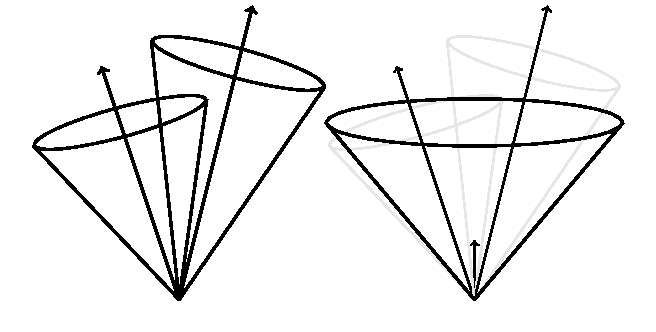
\includegraphics[width=0.45\textwidth]{figures/drawings/infrared_safety/jetinfrared.pdf}\hfill
    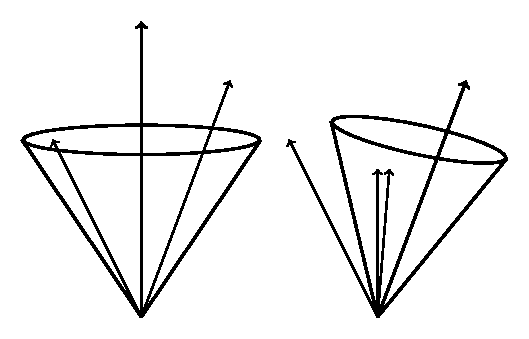
\includegraphics[width=0.45\textwidth]{figures/drawings/infrared_safety/jetcollinear.pdf}
    \caption[Effect of infrared emissions and collinear splittings on jet
    algorithms]{The influence of an infrared emission and a quasi
        collinear splitting on a jet algorithm not fulfilling the infrared safe
        and collinear safe requirements is shown. An additional soft particle (left plot)
    leads to the combination of the two jets into one large jet. A
quasi-collinear splitting of a particle (right plot) changes the result of the
jet clustering algorithm.}
    \label{fig:infrared_safety}
\end{figure}

\subsection{Generalized \kt Jet Algorithms}

The most popular sequential recombination algorithms are the \kt jet
algorithms. They cluster jets based on a jet size parameter $R$ and an
additional parameter $p$ which introduces a dependence on the transverse momentum of
the input objects. The pairwise algorithm uses a list of input objects which
can be partons, stable particles or reconstructed particle candidates.

First, the distance $d_{ij}$ between two particles $i$ and $j$ and the distances
$d_{iB}$ and $d_{jB}$ of the particles to the beam are calculated based on the
rapidity difference $\Delta y_{ij}$ and the azimuthal angle $\Delta \phi_{ij}$
between them:

\begin{align*} 
    d_{ij} &= \min(p_{\mathrm{T}i}^{2p},p_{\mathrm{T}j}^{2p})\frac{\left(\Delta
        R_{ij}\right)^2}{R^2}\\
    d_{i\mathrm{B}} &= k_{\mathrm{T}i}^{2p}
\end{align*} 
%
with the angular distance
%
\begin{align*}
    \left(\Delta R_{ij}\right)^2 &= (\Delta y_{ij})^2 + (\Delta \phi_{ij})^2
\end{align*} 
%
If the distance $d_{ij}$ is smaller than the distances to the beam line, the two
particles $i$ and $j$ are merged into a new particle $k$ which then replaces the
particles $i$ and $j$ in the input list. These steps are repeated until all
particles are clustered into jets. Since the distance measures are defined in
Minkowski space, the shapes of the jets in the $\eta$-$\phi$ plane are not circular but
irregular, see Figure~\ref{fig:jet_shapes}. Based on the parameter $p$, there
are three important \kt based algorithms with distinct properties:

\begin{figure}[htbp]
    \centering
    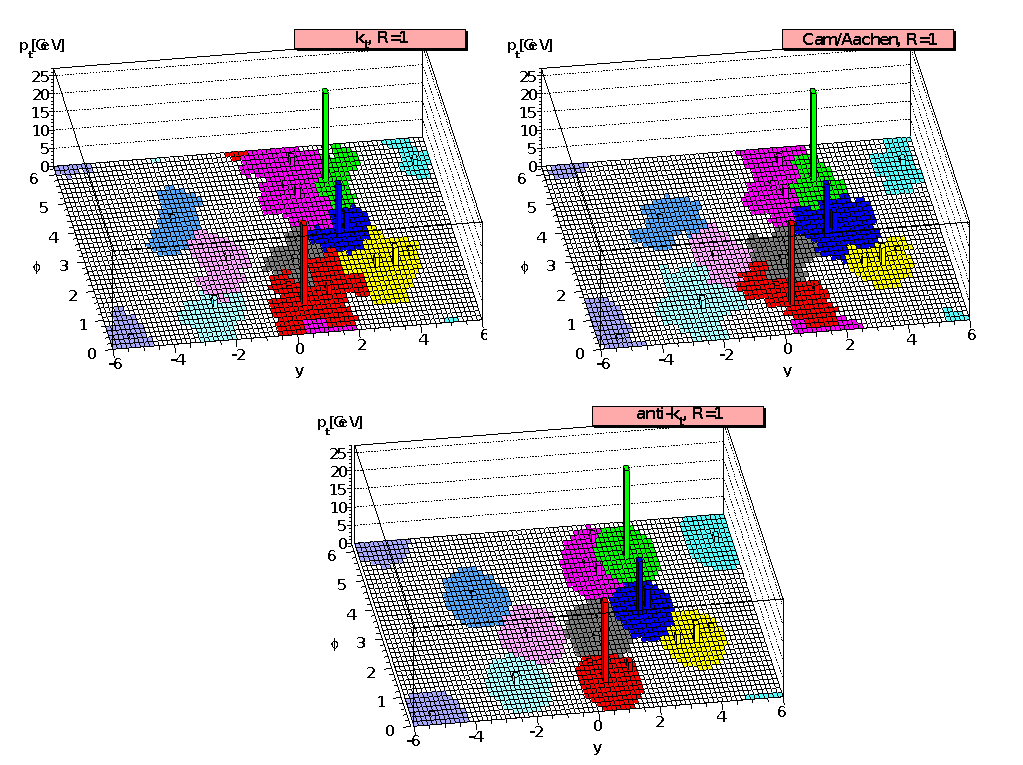
\includegraphics[width=0.8\textwidth]{figures/theoretical_foundations/jet_shapes.pdf}
    \caption[Jet areas of various jet algorithms]{Catchment areas of jets
        obtained by the described \kt-based algorithm. For most jet algorithms the shape is
        irregular, while the \antikt algorithm yields circular shapes for hard
        jets while and crescent-shaped soft jets. Adapted
        from~\cite{Salam:2009jx}.}
    \label{fig:jet_shapes}
\end{figure}

\begin{itemize}
    \item $p=1$: The \textbf{Inclusive $\mathbf{\kt}$
    algorithm}~\cite{Catani:1991hj,Catani:1992rm} is based on a \ptsq
        distance measure and approximately describes the inversion
        of the QCD branching process.\todo{ref}
    \item $p=0$: The \textbf{Cambridge-Aachen
        algorithm}~\cite{Dokshitzer:1997in} is only based on the spatial
        separation of the objects and does not rely on the transverse energy of
        the input objects. Similarly to the inclusive \kt algorithm, it produces
        jets of irregular shape. While it is not widely used for jet analyses,
        it is very interesting in the context of jet substructure studies, where
        at first a jet with a large jet size is clustered and subsequently its
        structure is investigated.
    \item  $p=-1$: The \textbf{anti-$\mathbf{\kt}$
    algorithm}~\cite{Cacciari:2008gp} favors clustering hard input objects
    resulting in fairly circular jet shapes for hard jets, while soft jets in
    close proximity to a reconstructed hard jet are crescent-shaped. It is the
    most widely used jet algorithm for physics analyses at the LHC.
\end{itemize}

\section{Dijet Production at Proton Colliders}

When two protons collide, the actual interaction takes place between the
constituents of the proton, the partons. The cross section $\sigma$ of such a hard
scattering process can be expressed in collinear factorization as

\begin{equation*}
    \begin{split}
    \sigma_{P_1 P_2 \rightarrow X} = &\sum_{i,j} \int dx_1 dx_2 f_{i, P_1}
    \left(x_1, \muf^2 \right) f_{j,P_2} \left(x_2, \muf^2 \right) \\ 
    &\times \hat\sigma_{i,j \rightarrow X} \left( x_1 p_1, x_2p_2, \as(\mur^2),
    \frac{Q^2}{\muf^2} \right),
\end{split}
\end{equation*}
%
where $f_i$ and $f_j$ denote the parton distributions, which depend on the
momentum fraction $x$ of the parent proton $P$ and the factorization scale
$\muf$. The parton-level cross section $\hat \sigma$ for the production of the
final state $X$ depends on the final state phase, the factorization scale and
the renormalization scale. The sum runs over all contributing initial state
partons. Fig.~\ref{fig:crosssection_factorization} illustrates the factorization
into the PDFs and the hard scattering cross section.

\begin{figure}[htbp]
    \centering
    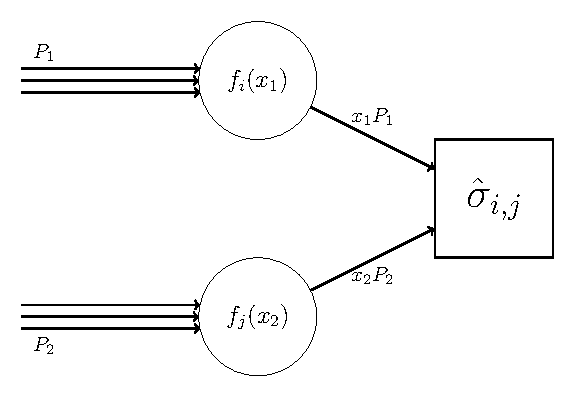
\includegraphics[width=0.5\textwidth]{figures/drawings/hardscattering.pdf}
    \caption[Factorization of hard scattering cross section.]
        {The total cross section is factorized into the hard scattering cross
        section $\hat \sigma$ and the PDFs $f_i(x)$.}
    \label{fig:crosssection_factorization}
\end{figure}

\subsection{Kinematics of the Dijet System}
\label{sec:dijet_kinematics}

The outgoing partons of a hard interaction manifest themselves as streams of
collimated particles which are clustered into jets. Consequently, the
properties of jets are studied in order to gain a deeper understanding of
QCD and the proton structure. In the following discussion, the incoming partons
involved in the scattering process are assumed to be massless and collinear to
the beam protons. Furthermore, it is convenient to describe the kinematics of
the dijet system using the transverse momentum \pt and the rapidity $y$ of the
jets, as it is introduced in Sec.~\ref{sec:coord_system}. The rapidity $y$, defined as

\begin{equation*}
    y = \frac{1}{2} \ln \left( \frac{E+p_z}{E-p_z} \right),
\end{equation*}
%
is at lowest order directly related to the proton momentum fractions $x_1$ and
$x_2$ via
%
\begin{equation*}
    x_1 = \frac{x_\mathrm{T}}{2} \left( e^{y_1} + e^{y_2} \right)
    \qquad\text{and}\qquad x_2 = \frac{x_\mathrm{T}}{2} \left( e^{-y_1} +
    e^{-y_2} \right),
\end{equation*}
%
\todo{herleitung}
with $x_{\mathrm{T}} = \pt/E$ and the rapidities $y_1$ and $y_2$ of the
two outgoing partons.


\begin{figure}[htbp]
    \centering
    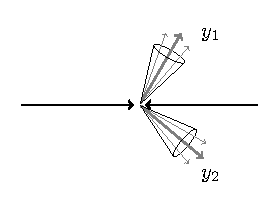
\includegraphics[width=0.45\textwidth]{figures/drawings/dijet_lab.pdf}
    \includegraphics[width=0.45\textwidth]{figures/drawings/dijet_cm.pdf}
    \caption[Dijet event in laboratory and center-of-mass frame.]
        {Dijet event in the laboratory frame (left) with the rapidities $y_1$
        and $y_2$ of the jets and in the center-of-mass frame (right) with the
    rapidities $\pm\ystar$.}
    \label{fig:dijet_cm_lab_frame}
\end{figure}

The longitudinal boost of the parton-parton center-of-mass (CM) frame with
respect to the proton-proton CM frame, \yboost, is calculated from the
rapidities $y_1$ and $y_2$ of the two jets emerging from the partons. 

\begin{equation*}
    \yboost = \frac{1}{2} |y_1 + y_2|
\end{equation*}

In the center-of-mass (CM) frame, the rapidities of the jets can be expressed
using the variable $\ystar$. As \ystar is symmetric, it is defined as

\begin{equation*}
    \ystar = \frac{1}{2} |y_1 - y_2|.
\end{equation*}

The quantity \ystar may also be expressed in terms of the polar scattering angle
$\theta^*$ with respect to the beamline by 

\begin{equation*}
    \ystar = \frac{1}{2} \ln \left( \frac{1 + |\cos \theta^*|}{1- | \cos \theta^*|} \right).
\end{equation*}

\todo{generell mehr ausführen.}
